\documentclass{standalone}
\usepackage{tikz}
\usetikzlibrary{calc}
\begin{document}
	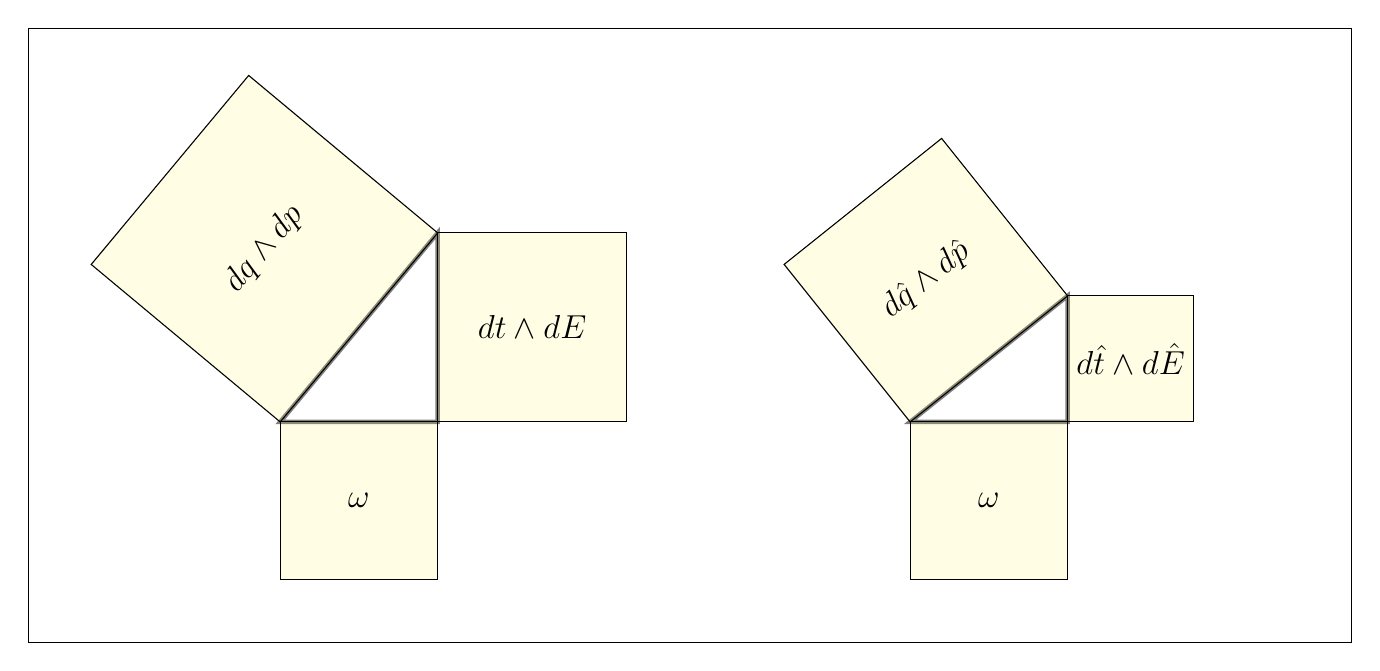
\begin{tikzpicture}[scale=0.4]
	
	
		% INPUTS:
		\newcommand{\avar}{5};		% omega horizontal length
		\newcommand{\bvar}{6};		% height of first dt dE 
		\newcommand{\dvar}{4};			 % height of second dt dE
		\newcommand{\xvar}{20};			% space between the two
		
	
		% styles
		\tikzstyle{triangle}=[ultra thick,fill=white,opacity=0.5];
		\tikzstyle{projection} = [fill=yellow,fill opacity=0.1,text opacity =1,text=black];
	
		% outer rectangle and name of diagram
		\draw (-8,-7) rectangle (34,12.5);
		
		% the different points that will be connected to draw the shapes
		\coordinate (p2) at (\avar,0);
		\coordinate (p3) at (\avar,\bvar);
		\coordinate (p5) at (\avar + \bvar,\bvar);	
	    \coordinate (p7) at (\avar,- \avar);
	    \coordinate (p8) at (\avar - \bvar,\avar + \bvar);

		% angle made by the coordinates to rotate the first dq dp square
		\newcommand{\thetavar}{atan2(\bvar , \avar)};
		
		% drawing the first shape
		\filldraw[style=triangle] (0,0) -- ($(p2)$) -- ($(p3)$) -- cycle;
		
		\filldraw[style=projection,rotate around={0:(0,0)}] (0,0) rectangle ($(p7)$) node[pos=.5] {\large $\omega$};
				
		\draw[style=projection,rotate around={\thetavar:(0,0)}] (0,0) rectangle ($(p8)$) node[pos=.5, rotate=\thetavar] {\large $dq\wedge dp$};
			
		\draw[style=projection,rotate around={0:(0,0)}] ($(p2)$) rectangle ($(p5)$) node[pos=.5] {\large $dt\wedge dE$};	
		
		% coordinates to the second shape (to the right)
		\coordinate (h0) at (\xvar,0);
		\coordinate (h2) at (\xvar + \avar,0); 
		\coordinate (h3) at (\xvar + \avar, \dvar);
		\coordinate (h5) at (\xvar + \avar + \dvar, \dvar);
		\coordinate (h7) at (\xvar + \avar,- \avar);
		\coordinate (h8) at (\xvar + \avar - \dvar,\avar + \dvar);

		% angle made by the coordinates to rotate the first dq dp square
		\newcommand{\phivar}{atan2(\dvar , \avar)};

		%drawing the shape on the right
		\filldraw[style=triangle] ($(h0)$) -- ($(h2)$) -- ($(h3)$) -- cycle;

		\filldraw[style=projection,rotate around={0:($(h0)$)}] ($(h0)$) rectangle ($(h7)$) node[pos=.5] {\large $\omega$};

		\draw[style=projection,rotate around={\phivar:($(h0)$)}] ($(h0)$) rectangle ($(h8)$) node[pos=.5, rotate=\phivar] {\large $d\hat{q}\wedge d\hat{p}$};

		\draw[style=projection,rotate around={0:($(h0)$)}] ($(h2)$) rectangle ($(h5)$) node[pos=.5] {\large $d\hat{t}\wedge d\hat{E}$};

		
	\end{tikzpicture}
\end{document}